% Chương 4 — phần giao diện/demo (Trúc). Ghép vào cuối \chapter{Kết quả và phân tích}.
% Nguồn: BA/*.md, reports/P13-full-flow-audit-2026-10-31.md, SERVER_CONTEXT/chapter4_evidence.md (nhánh thesis),
% ảnh chụp 05/11/2026 từ stack Docker nhánh dev (commit 1a8a767).
% Phần này trả lời câu hỏi: điểm số của mô hình được đưa vào quy trình chăm sóc khách hàng như thế nào.
% Chia việc Ch.4: Quân (EDA, dữ liệu) · Trung (hệ thống/API) · Huy (bảng metric) · Trúc (giao diện/demo).
% Không lặp kiến trúc/API (phần Trung) và kết quả kiểm thử web (để ở báo cáo kiểm thử, không đưa vào khóa luận ML).

\section{Ứng dụng điểm rủi ro vào quy trình chăm sóc khách hàng}\label{sec:demo}

Một điểm rủi ro chỉ tạo ra giá trị khi nó thay đổi việc nhân viên làm tiếp theo. Mục này trình bày cách đầu ra của luồng học máy ở Chương~\ref{ch:method} được đưa vào ứng dụng vận hành: điểm số biến thành thứ tự ưu tiên ra sao, người dùng đọc và diễn giải điểm số ở đâu, và hệ thống ghi lại những gì để đánh giá mô hình về sau. Hai phần minh họa cuối mục cho thấy luật tổng hợp và ngưỡng ưu tiên làm thay đổi danh sách đơn ra sao. Dữ liệu đầu vào và kiến trúc hệ thống được trình bày ở các mục khác của chương này nên không nhắc lại.

Cần nói rõ ngay từ đầu: điểm số trong bản demo \emph{không} phải là kết quả suy luận của mô hình rừng ngẫu nhiên được giữ lại ở mục trước. Bản demo dùng 100 đơn Olist thật (thông tin đơn, người bán, danh mục) gắn với điểm minh họa có tính tất định, cùng 5 đơn giả lập; phiên bản mô hình hiển thị trên giao diện là \texttt{olist-ui-demo-v1}. Lý do và hệ quả của lựa chọn này được phân tích ở mục~\ref{sec:demo-limits}. Vì vậy, mục này đánh giá \emph{cách hệ thống sử dụng điểm số}, không đánh giá chất lượng của điểm số.

% ---------------------------------------------------------------------
\subsection{Từ điểm số đến hàng đợi ưu tiên}

Giữa luồng học máy và ứng dụng chỉ có một điểm nối là bảng dự đoán trong cơ sở dữ liệu (Hình~\ref{fig:arch}). Mỗi lần chấm điểm theo lô tạo ra một \emph{snapshot dự đoán} bất biến, gồm điểm của từng item, điểm của đơn tổng hợp theo luật max-v1 (Phương trình~\ref{eq:maxv1}), mức rủi ro theo ngưỡng của phiên bản mô hình, các yếu tố liên quan và các mã phiên bản. Tại mỗi thời điểm chỉ một snapshot ở trạng thái hoạt động. Ứng dụng đọc snapshot này để tạo các \emph{case} cần xử lý; mỗi case giữ mã dự đoán và luật tổng hợp tại thời điểm được tạo, nên khi mô hình được chấm lại, các case đang mở vẫn được xử lý theo đúng điểm số đã sinh ra chúng thay vì bị đổi điểm giữa chừng.

Hình~\ref{fig:ui-queue} là hàng đợi rủi ro của nhân viên chăm sóc khách hàng. Ba quyết định thiết kế ở đây xuất phát trực tiếp từ đặc điểm của mô hình:

\begin{itemize}
  \item \textbf{Xếp theo điểm, sau đó theo hạn xử lý.} Đơn được sắp theo điểm rủi ro giảm dần, rồi theo hạn SLA gần nhất và thời gian chờ. Điểm số chỉ có ý nghĩa thứ tự (mục~\ref{sec:eval}), nên giao diện dùng nó để sắp xếp chứ không biến nó thành nhãn ``sẽ bị đánh giá thấp''.
  \item \textbf{Hiện sản phẩm có điểm cao nhất ngay trên dòng của đơn.} Cột ``Sản phẩm cần kiểm tra'' cho biết item quyết định điểm của đơn theo luật max-v1, kèm số sản phẩm còn lại. Nhân viên biết nên hỏi khách về sản phẩm nào trước, đồng thời thấy được điểm của đơn đến từ đâu.
  \item \textbf{Mức rủi ro quyết định ai xử lý.} Đơn mức cao do quản lý phân công, đơn mức trung bình và thấp nhân viên tự nhận. Ngưỡng rủi ro vì vậy là một quy tắc phân bổ nguồn lực chứ không chỉ là nhãn hiển thị, đúng với lập luận chọn ngưỡng theo năng lực xử lý ở mục~\ref{sec:models}.
\end{itemize}

\begin{figure}[htbp]\centering
  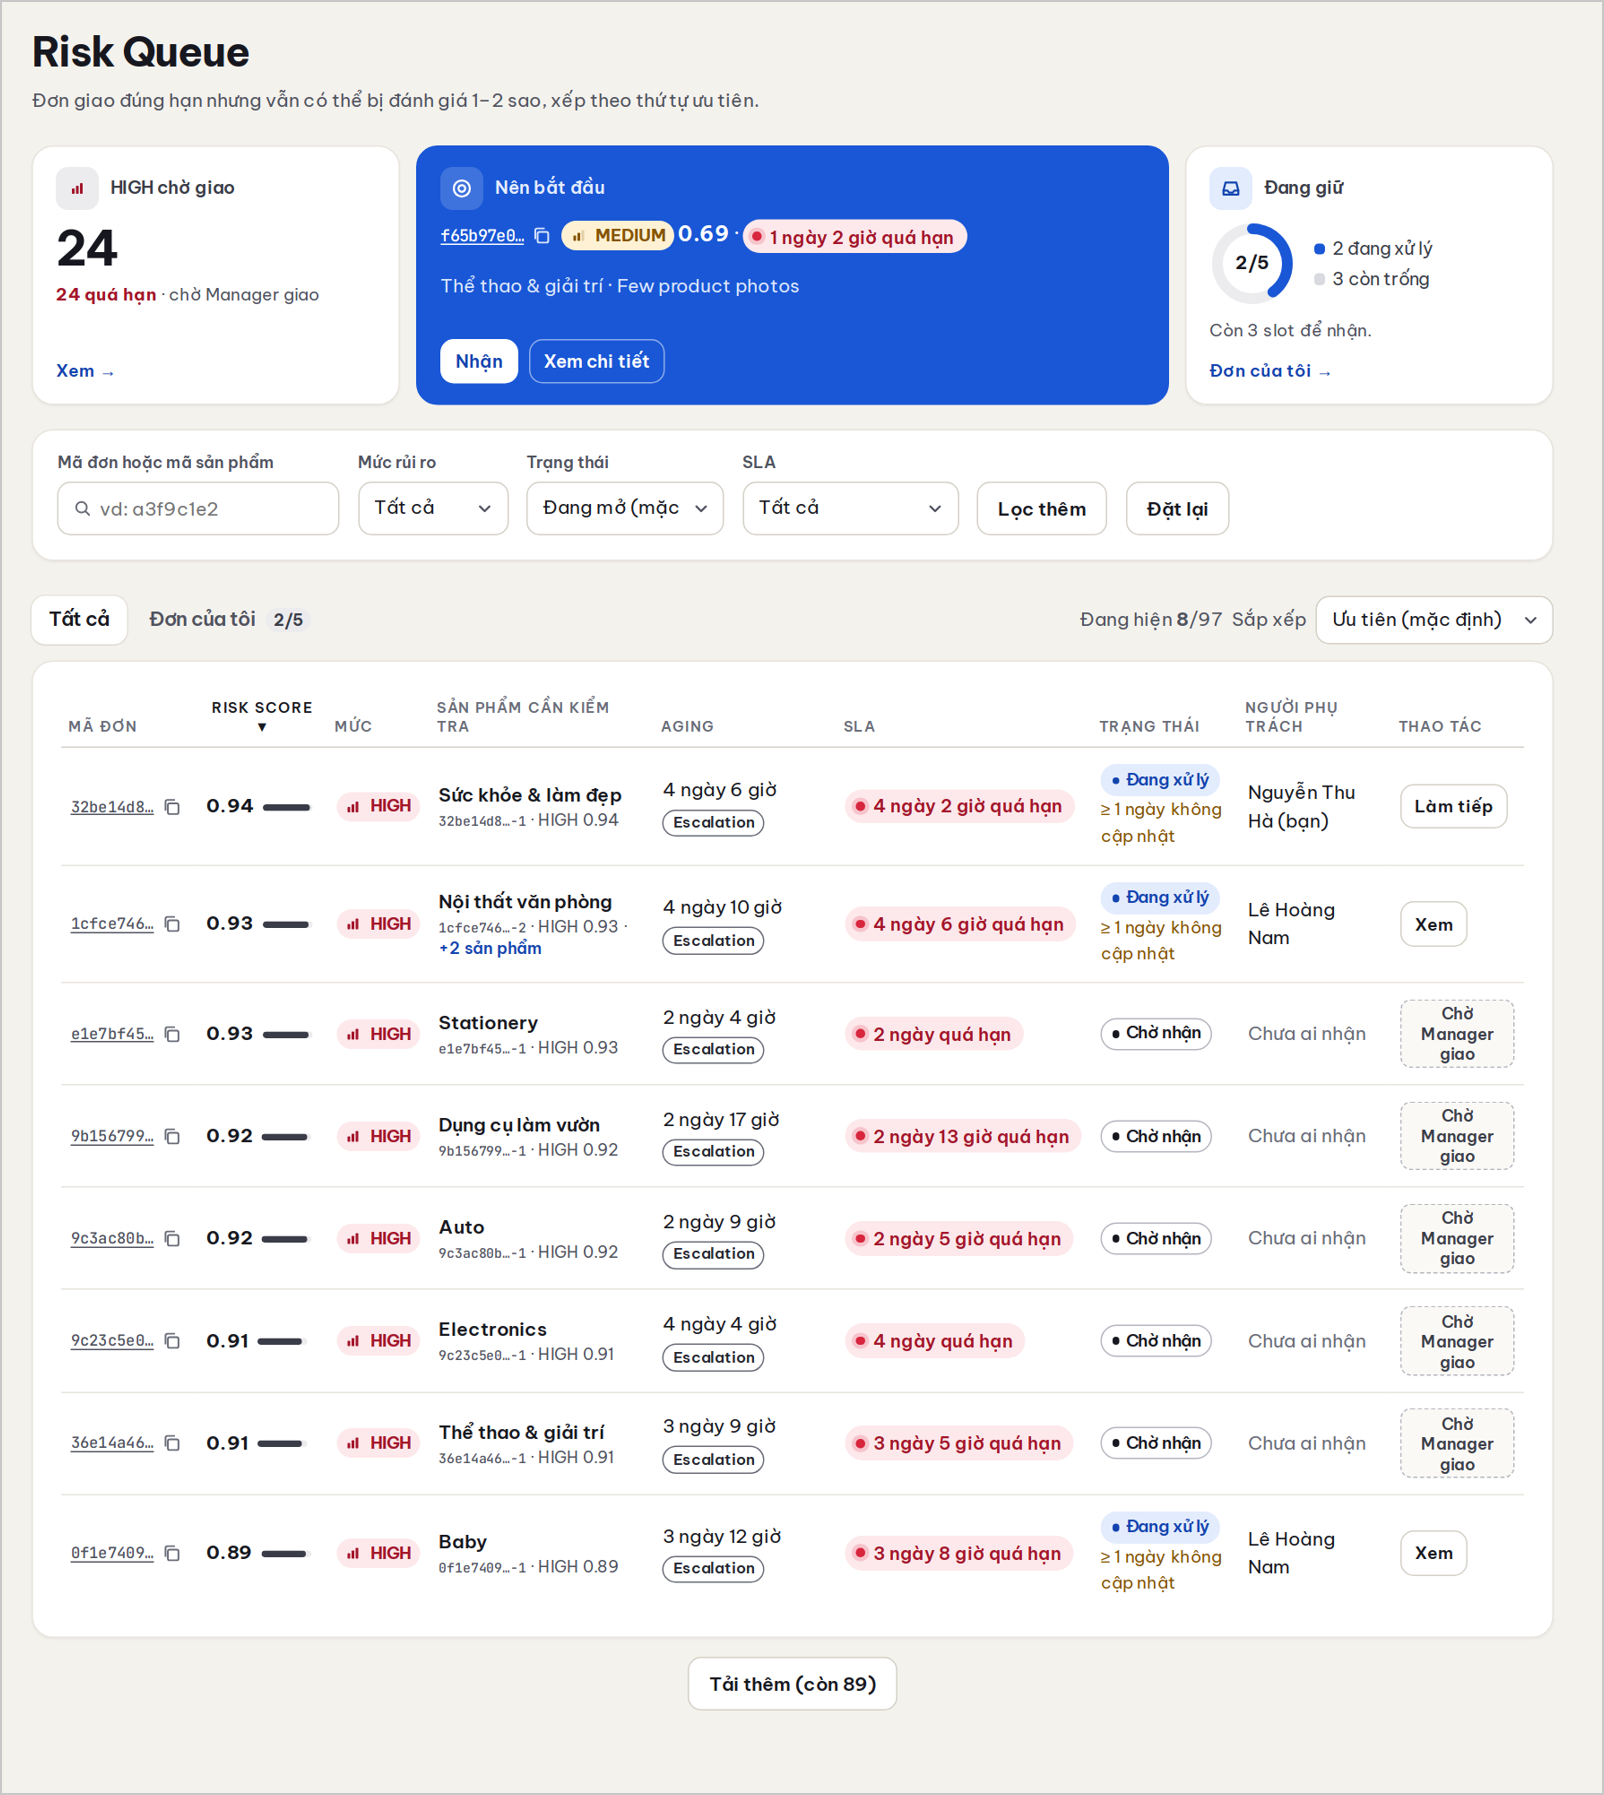
\includegraphics[width=\linewidth]{ui-risk-queue}
  \caption{Hàng đợi rủi ro của nhân viên: đơn sắp theo điểm, kèm sản phẩm có điểm cao nhất của mỗi đơn (dữ liệu demo).}\label{fig:ui-queue}
\end{figure}

% ---------------------------------------------------------------------
\subsection{Diễn giải điểm số ở mức đơn hàng}

Trang chi tiết đơn (Hình~\ref{fig:ui-detail}) là nơi người dùng đọc điểm số kỹ nhất, nên cũng là nơi dễ diễn giải sai nhất. Khối ``Kết quả model của đơn'' hiển thị bốn thông tin đi cùng điểm số: thanh điểm có vạch ngưỡng của mức trung bình và mức cao, luật tổng hợp, phiên bản mô hình và thời điểm dự báo, phiên bản ngưỡng. Bốn thông tin này giúp mọi con số trên màn hình truy ngược được về đúng lần chấm điểm đã sinh ra nó, cùng nguyên tắc với việc lưu cấu hình và mã commit của từng lần huấn luyện ở mục~\ref{sec:data}.

Ngay dưới điểm số là một câu nhắc cố định: điểm rủi ro dùng để ưu tiên kiểm tra, không phải kết luận khách không hài lòng. Câu nhắc này đến từ hai giới hạn đã nêu ở Chương~\ref{ch:method}. Thứ nhất, nhãn yếu ở mức item: điểm của sản phẩm là rủi ro đơn bị đánh giá thấp \emph{khi có mặt} sản phẩm đó, không phải bằng chứng sản phẩm gây ra bất mãn. Thứ hai, chỉ số đánh giá đo khả năng xếp hạng, không đo xác suất đúng của từng đơn.

Bảng sản phẩm trong đơn cho thấy điểm của từng item, và khối ``Yếu tố liên quan tới score'' được dành cho giải thích ở mức item. Trong bản demo, một số item có danh sách yếu tố minh họa đi kèm điểm số (Hình~\ref{fig:ui-multi}), số còn lại hiển thị ``chưa có giải thích''. Các yếu tố này là nhãn minh họa của dữ liệu demo, không phải giá trị SHAP; khối này là chỗ dành sẵn cho bước giải thích mô hình khi được thực hiện (mục~\ref{sec:demo-limits}). Hai chi tiết thiết kế giữ cho phần giải thích không bị đọc sai: khi thiếu giải thích, giao diện nói rõ là chưa có thay vì để trống, để người dùng không hiểu nhầm là đơn không có yếu tố rủi ro nào; khi có giải thích, ngay bên dưới luôn có câu ``các yếu tố này đi kèm điểm cao, không chứng minh nguyên nhân'', nhất quán với cách diễn giải giá trị SHAP như cách mô hình sử dụng đặc trưng chứ không phải tác động nhân quả.

\begin{figure}[htbp]\centering
  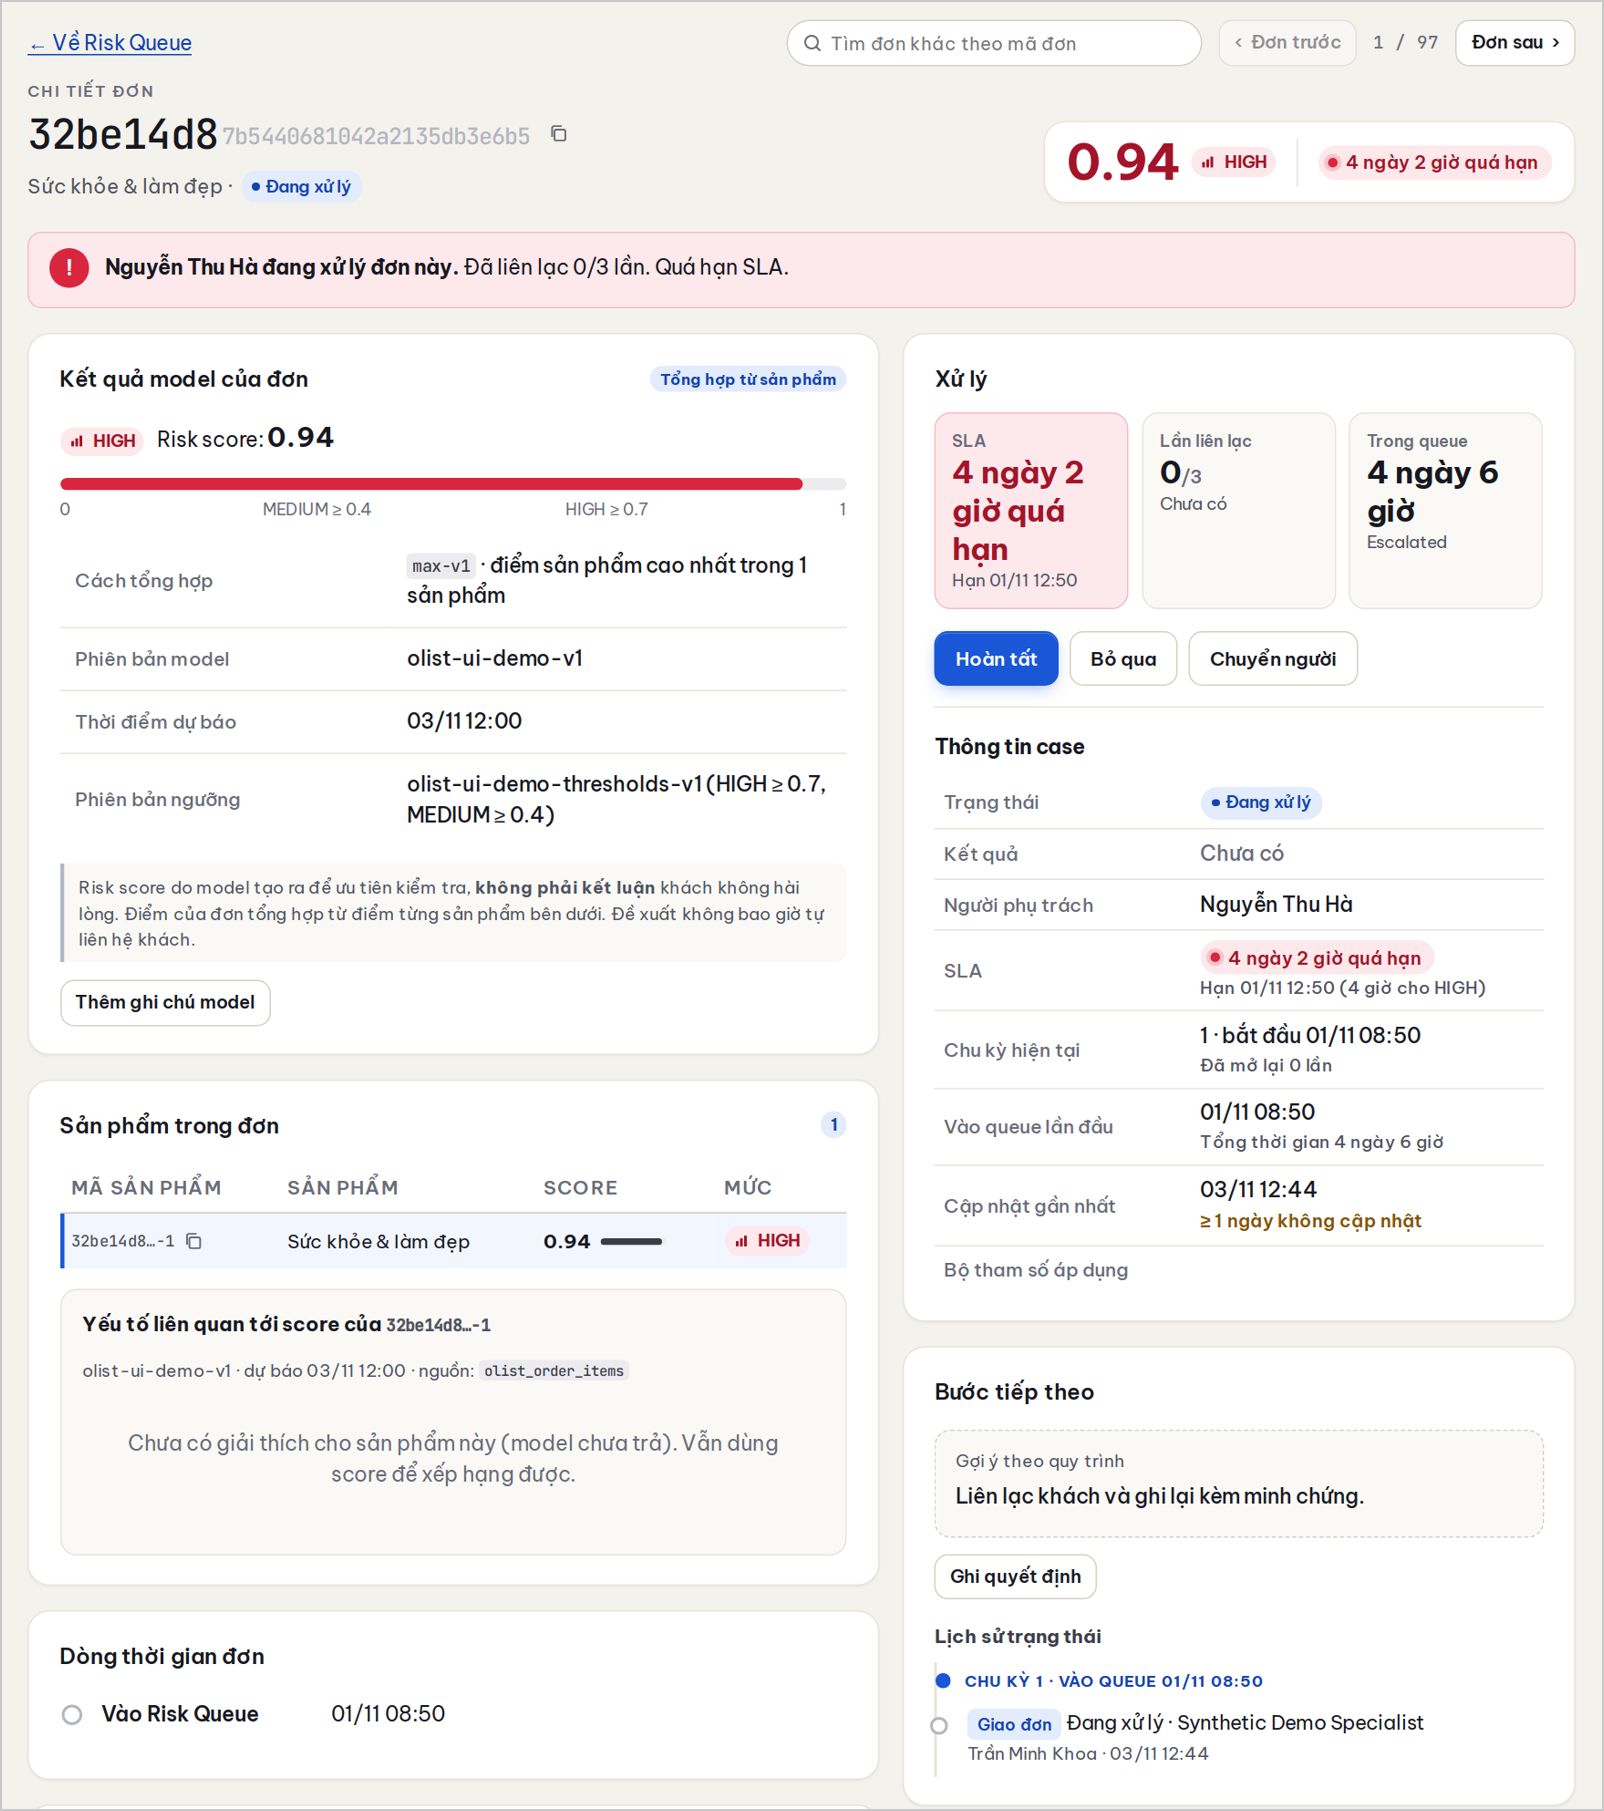
\includegraphics[width=\linewidth]{ui-order-detail}
  \caption{Chi tiết đơn: điểm số kèm vạch ngưỡng, luật tổng hợp, phiên bản mô hình và ngưỡng; điểm của từng sản phẩm (dữ liệu demo).}\label{fig:ui-detail}
\end{figure}

% ---------------------------------------------------------------------
\subsection{Theo dõi phân bố rủi ro}

Màn tổng quan của quản lý (Hình~\ref{fig:ui-dashboard}) tổng hợp số case theo mức rủi ro, theo ngày vào hàng đợi và theo khoảng điểm. Ngoài mục đích điều phối công việc, các khối này là công cụ quan sát đơn giản cho đầu ra của mô hình: nếu tỉ lệ đơn mức cao hoặc số case mới mỗi ngày thay đổi đột ngột giữa hai lần chấm điểm, quản lý thấy ngay mà không cần đọc báo cáo kỹ thuật. Như Bảng~\ref{tab:split} đã cho thấy, tỉ lệ dương dao động từ 10\% đến gần 14\% giữa các giai đoạn, nên việc theo dõi phân bố theo thời gian là cần thiết khi mô hình được dùng lâu dài.

Phần ``Xem theo khoảng score'' (Hình~\ref{fig:ui-bands}) chia các đơn theo năm khoảng điểm. Với dữ liệu demo, các khoảng gần như đều nhau: 15, 20, 26, 26 và 18 đơn từ khoảng thấp nhất tới cao nhất, tức điểm trung bình khoảng 0,52. Nếu đây là xác suất đã hiệu chỉnh, nó ngụ ý khoảng một nửa số đơn giao đúng hạn sẽ bị đánh giá thấp, trong khi tỉ lệ thực tế chỉ khoảng 10\%. Với một mô hình được hiệu chỉnh tốt, trung bình xác suất dự đoán phải xấp xỉ tỉ lệ dương, nên phần lớn đơn phải dồn về các khoảng điểm thấp. Vì vậy, bảng khoảng điểm là một phép kiểm tra nhanh mà quản lý tự làm được: nếu điểm trung bình lệch xa tỉ lệ đơn bị đánh giá thấp quan sát được, hoặc hình dạng phân bố thay đổi mạnh giữa hai lần chấm điểm, thì cần xem lại bước hiệu chỉnh hoặc dữ liệu đầu vào.

\begin{figure}[htbp]\centering
  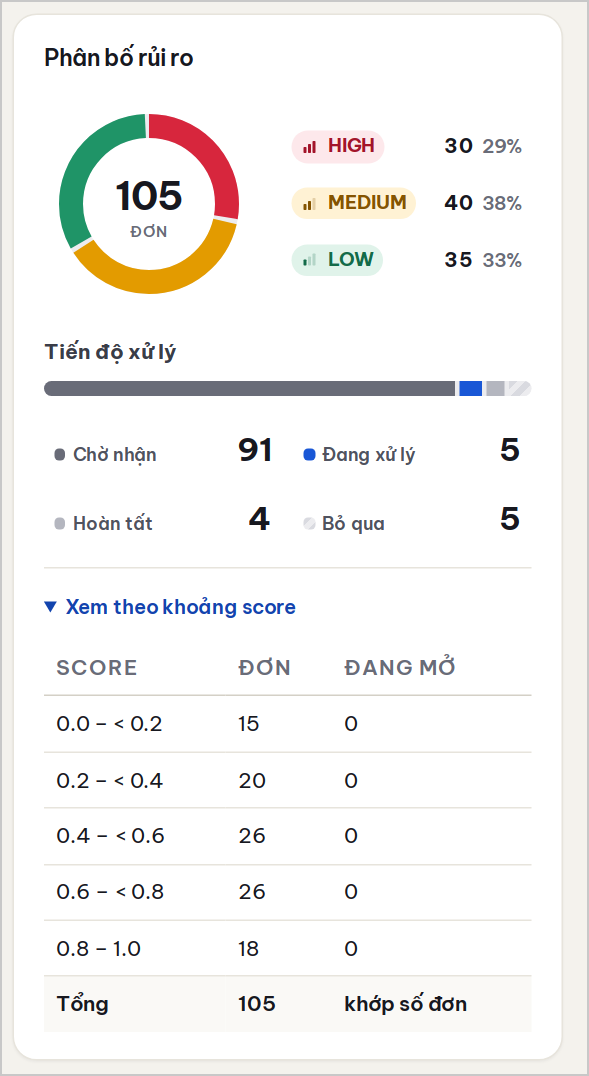
\includegraphics[width=0.45\linewidth]{ui-score-bands}
  \caption{Phân bố rủi ro và số đơn theo khoảng điểm (dữ liệu demo, điểm minh họa).}\label{fig:ui-bands}
\end{figure}

Chế độ ``Theo sản phẩm'' (Hình~\ref{fig:ui-product}) chuyển cùng các khối thống kê sang đơn vị item: 105 đơn trong bản demo gồm 114 sản phẩm, và danh sách sản phẩm có điểm cao nhất cho biết rủi ro tập trung ở danh mục nào. Hai chế độ tương ứng với hai đơn vị đã tách ở mục~\ref{sec:pipeline}: mô hình học và chấm điểm ở mức item, còn nhân viên xử lý ở mức đơn. Đặt hai góc nhìn cạnh nhau giúp người đọc không nhầm số sản phẩm rủi ro với số đơn cần liên hệ.

\begin{figure}[htbp]\centering
  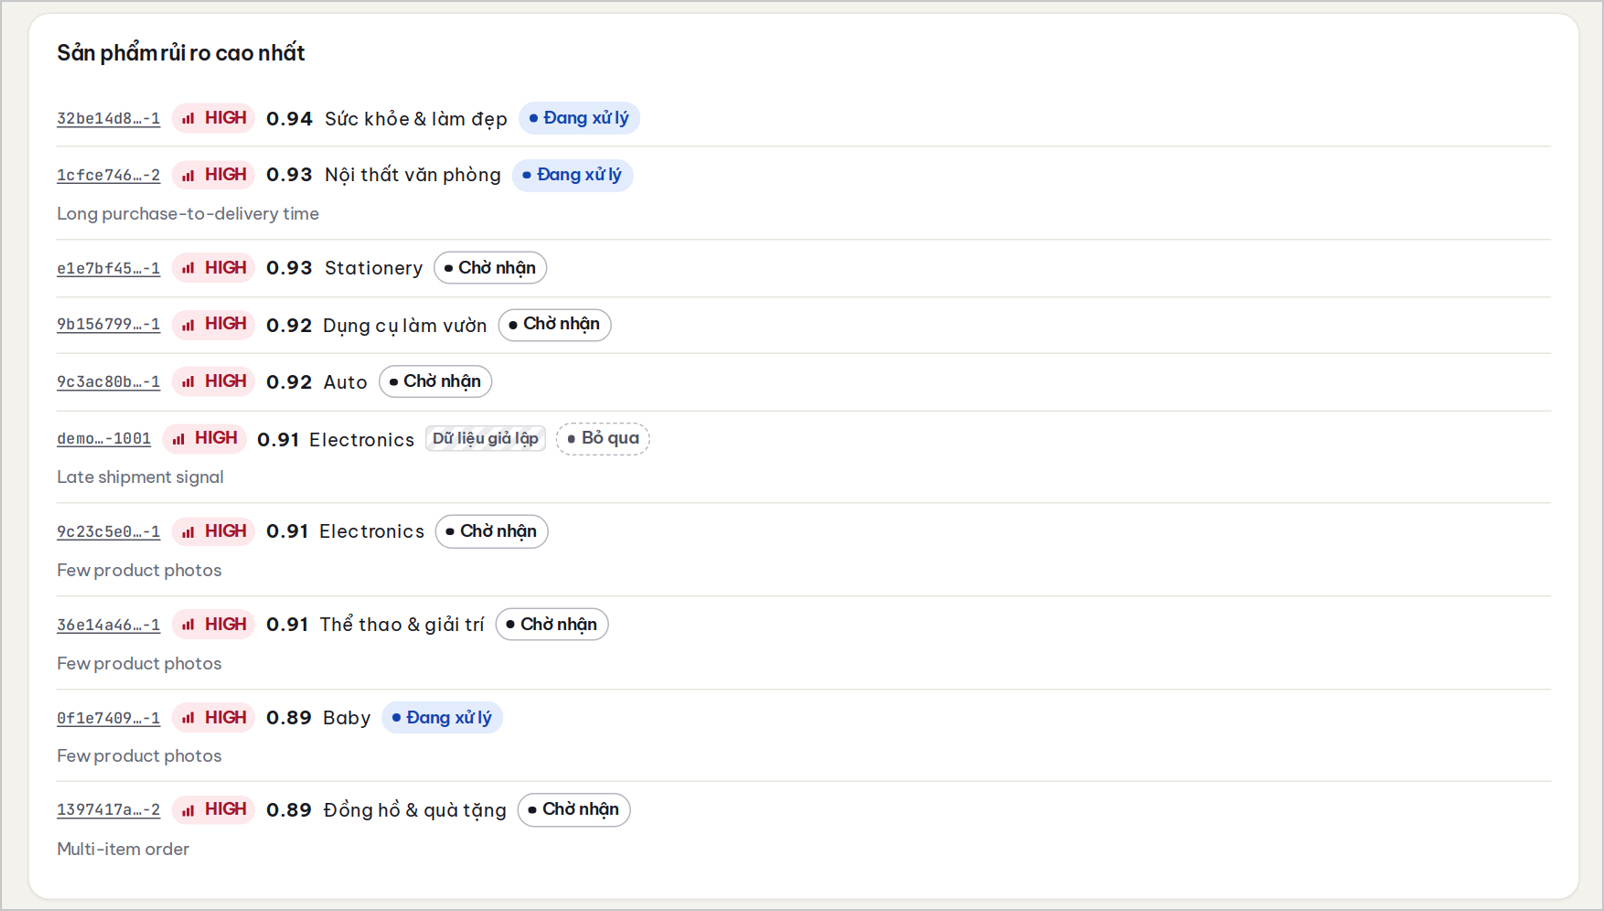
\includegraphics[width=\linewidth]{ui-product-view}
  \caption{Chế độ xem theo sản phẩm: các item có điểm cao nhất kèm danh mục và yếu tố minh họa (dữ liệu demo).}\label{fig:ui-product}
\end{figure}

Hình~\ref{fig:ui-dashboard} cũng minh họa trực quan giới hạn quan trọng nhất của bản demo: với ngưỡng cố định 0,7 và 0,4, mức HIGH chiếm 29\% số case, trong khi chính sách ở mục~\ref{sec:models} chỉ dành mức này cho 5\% đơn có điểm cao nhất. Điểm này được phân tích ở mục~\ref{sec:demo-limits} và Chương~5.

\begin{figure}[htbp]\centering
  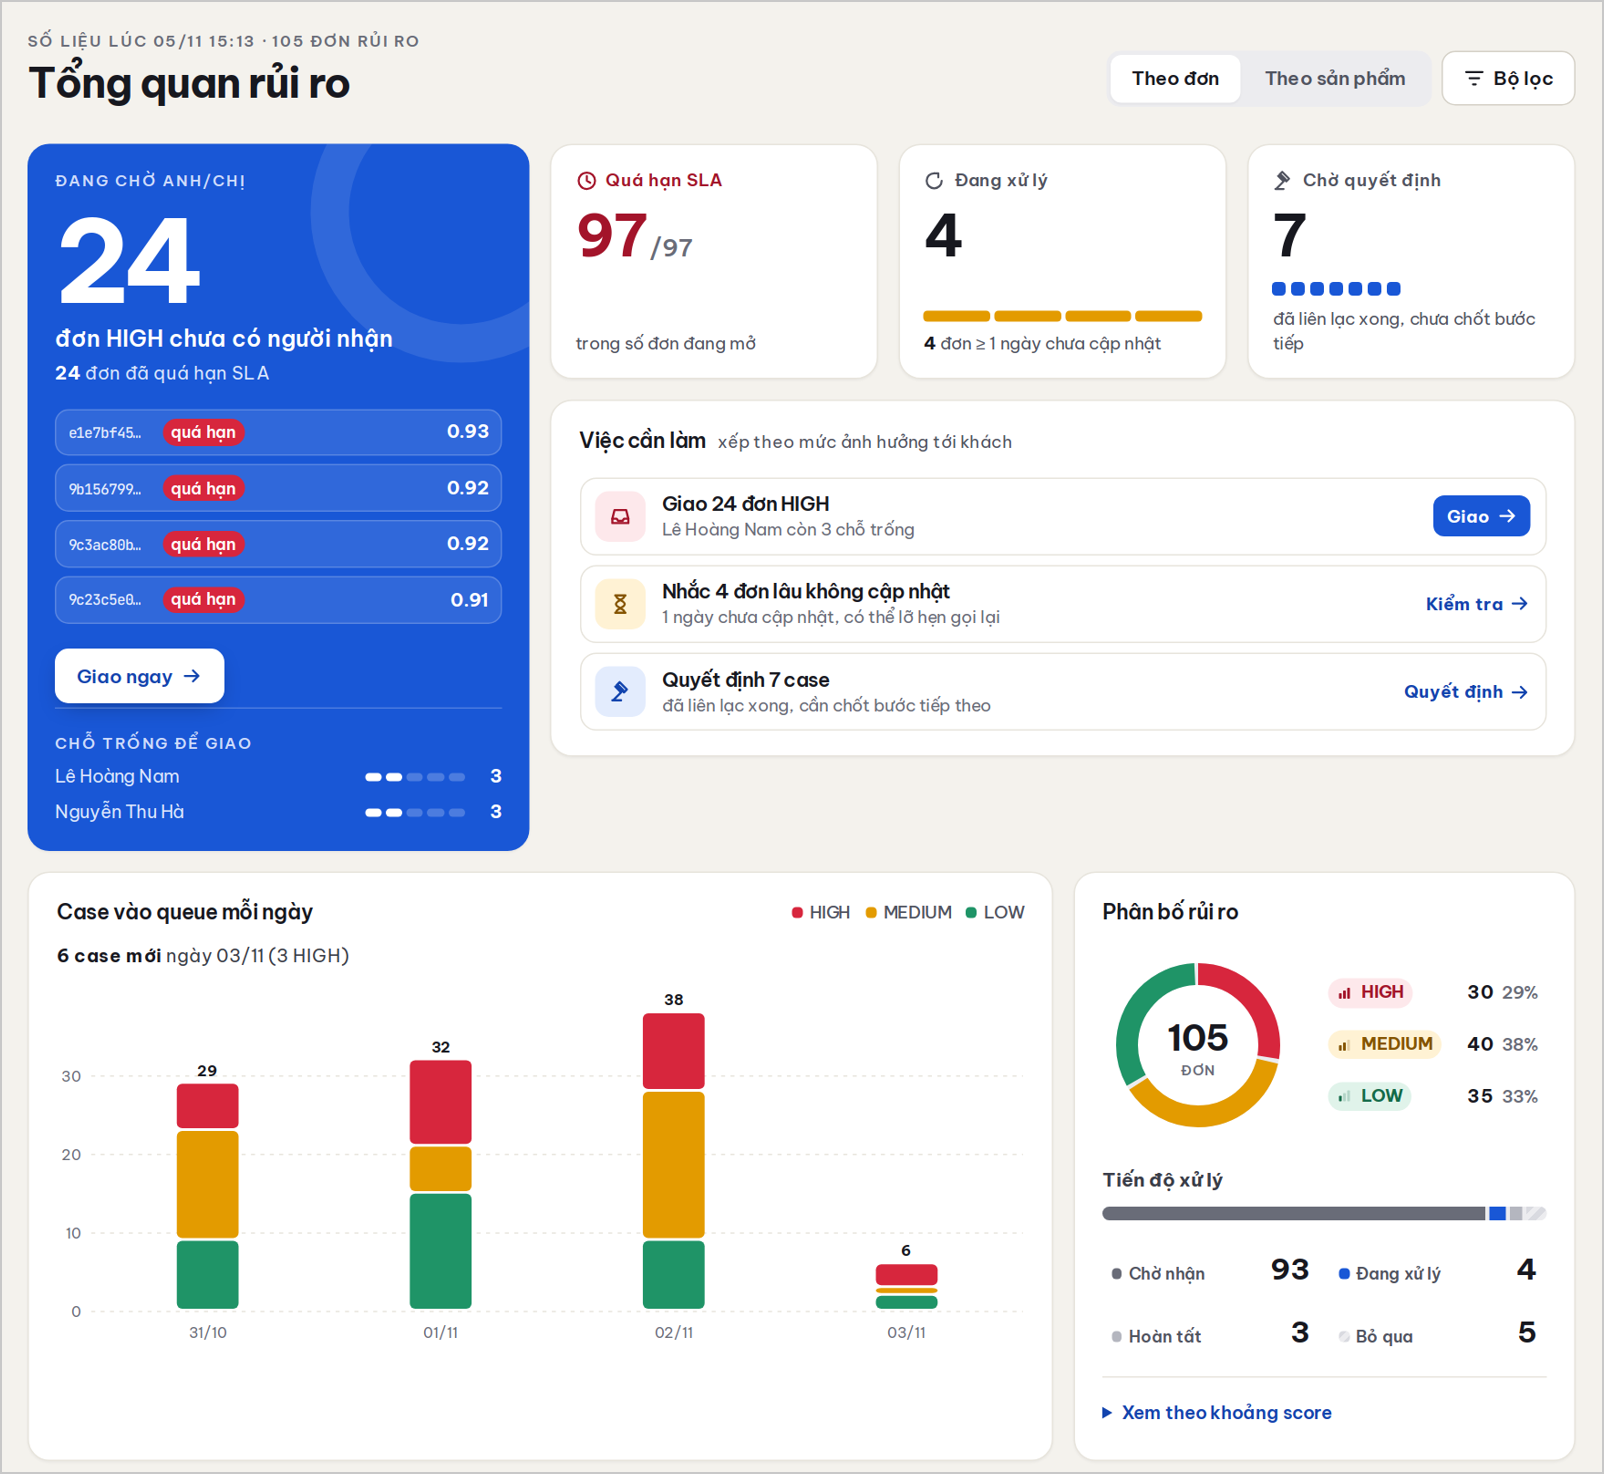
\includegraphics[width=\linewidth]{ui-dashboard}
  \caption{Tổng quan rủi ro của quản lý: case theo ngày và theo mức rủi ro (dữ liệu demo, ngưỡng cố định 0,7/0,4).}\label{fig:ui-dashboard}
\end{figure}

% ---------------------------------------------------------------------
\subsection{Dữ liệu vận hành phục vụ đánh giá mô hình}

Như đã nêu ở mục~\ref{sec:eval}, các chỉ số hiện tại chỉ đo khả năng dự báo, chưa đo hiệu quả can thiệp. Ứng dụng được thiết kế để tích lũy đúng loại dữ liệu cần cho bước đánh giá đó, theo ba nguyên tắc:

\begin{enumerate}
  \item \textbf{Điểm số chỉ đọc.} Không có thao tác nào sửa điểm hay mức rủi ro. Quản lý có thể thêm ghi chú về mô hình cho một đơn, nhưng ghi chú được lưu riêng. Nhờ vậy, sau này có thể so sánh điểm gốc với kết quả thực tế mà không lo điểm đã bị chỉnh tay.
  \item \textbf{Kết quả xử lý có cấu trúc.} Khi đóng case, nhân viên phải chọn một kết quả trong danh mục cố định (có vấn đề, không có vấn đề, trùng case) hoặc một lý do bỏ qua (không liên lạc được, khách từ chối, \ldots). Mỗi lần liên lạc được ghi lại với cách liên lạc và kết quả. Kết quả ``có vấn đề'' và ``không có vấn đề'' là một nguồn nhãn độc lập với đánh giá sao, có thể dùng để đo precision của nhóm HIGH trong vận hành thật.
  \item \textbf{Lịch sử chỉ thêm, không sửa.} Mọi thao tác đều được ghi lại với thời điểm và người thực hiện, nên có thể dựng lại đơn nào đã được liên hệ, khi nào, sau bao lâu kể từ lúc có điểm, để đối chiếu với nhãn quan sát được về sau.
\end{enumerate}

Mỗi lần liên hệ được ghi qua màn hình liên lạc khách (Hình~\ref{fig:ui-contact}) với thời điểm, phương thức, kết quả và ngày hẹn liên hệ tiếp. Đây là bản ghi \emph{can thiệp}, phần dữ liệu mà bộ Olist không có. Khi dùng để đánh giá, cần tách hai trường hợp dễ bị gộp chung: nếu sau số lần liên hệ tối đa vẫn không gặp được khách, case tự chuyển sang bỏ qua với lý do ``không liên lạc được'', nghĩa là can thiệp \emph{chưa xảy ra}; trường hợp này khác với can thiệp đã xảy ra nhưng khách vẫn đánh giá thấp. Gộp hai nhóm sẽ làm hiệu quả can thiệp trông thấp hơn thực tế.

\begin{figure}[htbp]\centering
  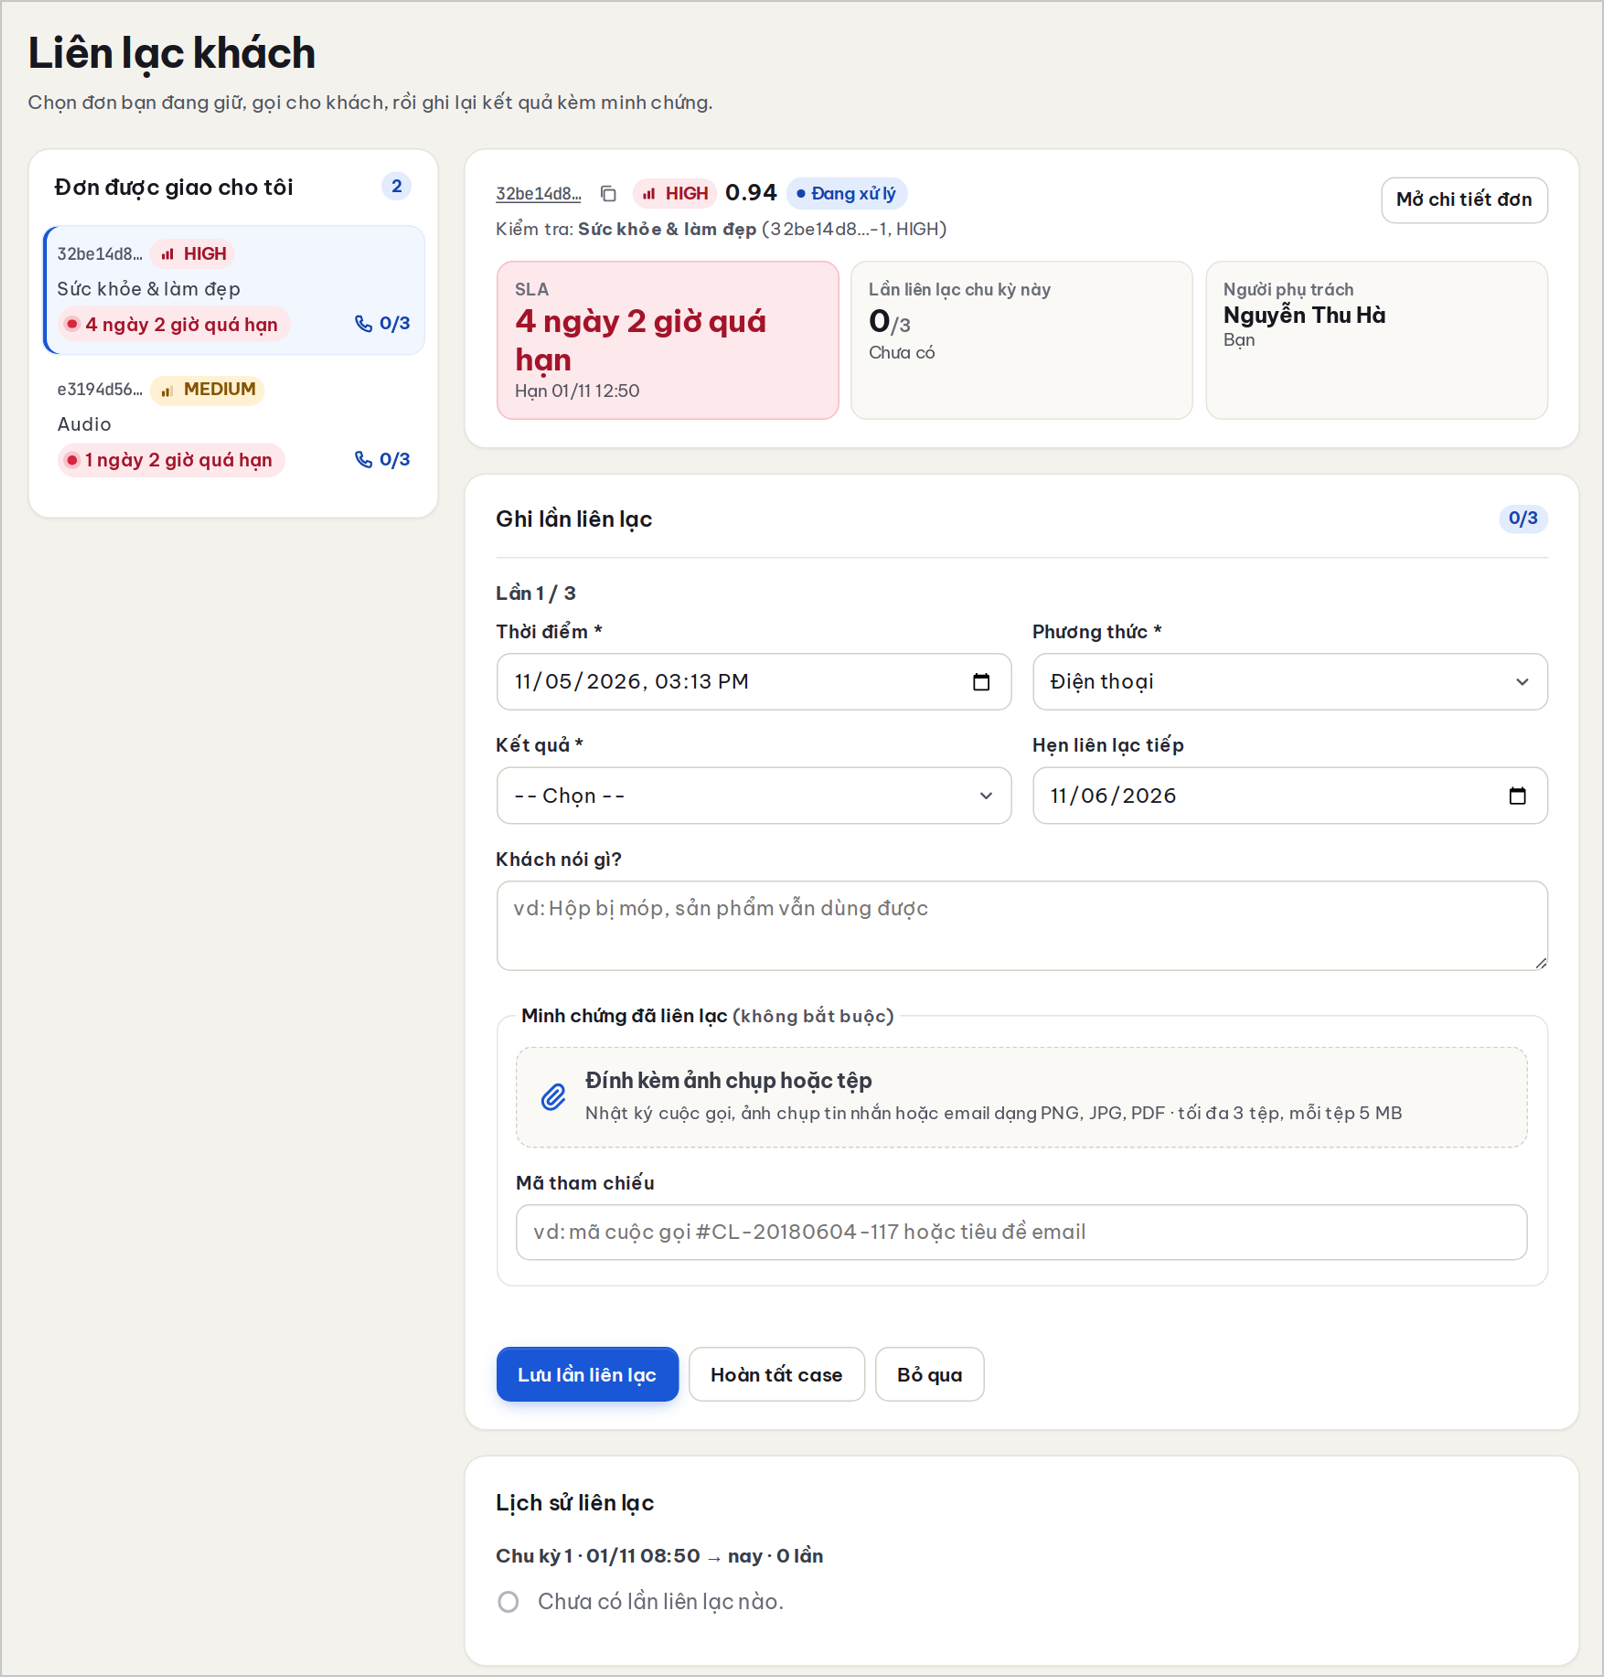
\includegraphics[width=\linewidth]{ui-contact-attempt}
  \caption{Màn hình liên lạc khách: mỗi lần liên hệ được ghi với thời điểm, phương thức, kết quả và minh chứng (dữ liệu demo).}\label{fig:ui-contact}
\end{figure}

Hình~\ref{fig:ui-closed} là một case đã đóng: điểm 0,68 ở mức trung bình nằm cạnh kết quả xử lý ``có vấn đề'', lần liên lạc và quyết định tiếp theo của quản lý. Mỗi case đóng như vậy là một cặp \emph{(điểm dự báo, kết quả quan sát)} gắn với đúng phiên bản mô hình đã sinh ra điểm. Hình~\ref{fig:feedback-loop} tóm tắt cách các cặp này quay lại phục vụ đánh giá và cải tiến mô hình.

\begin{figure}[htbp]\centering
  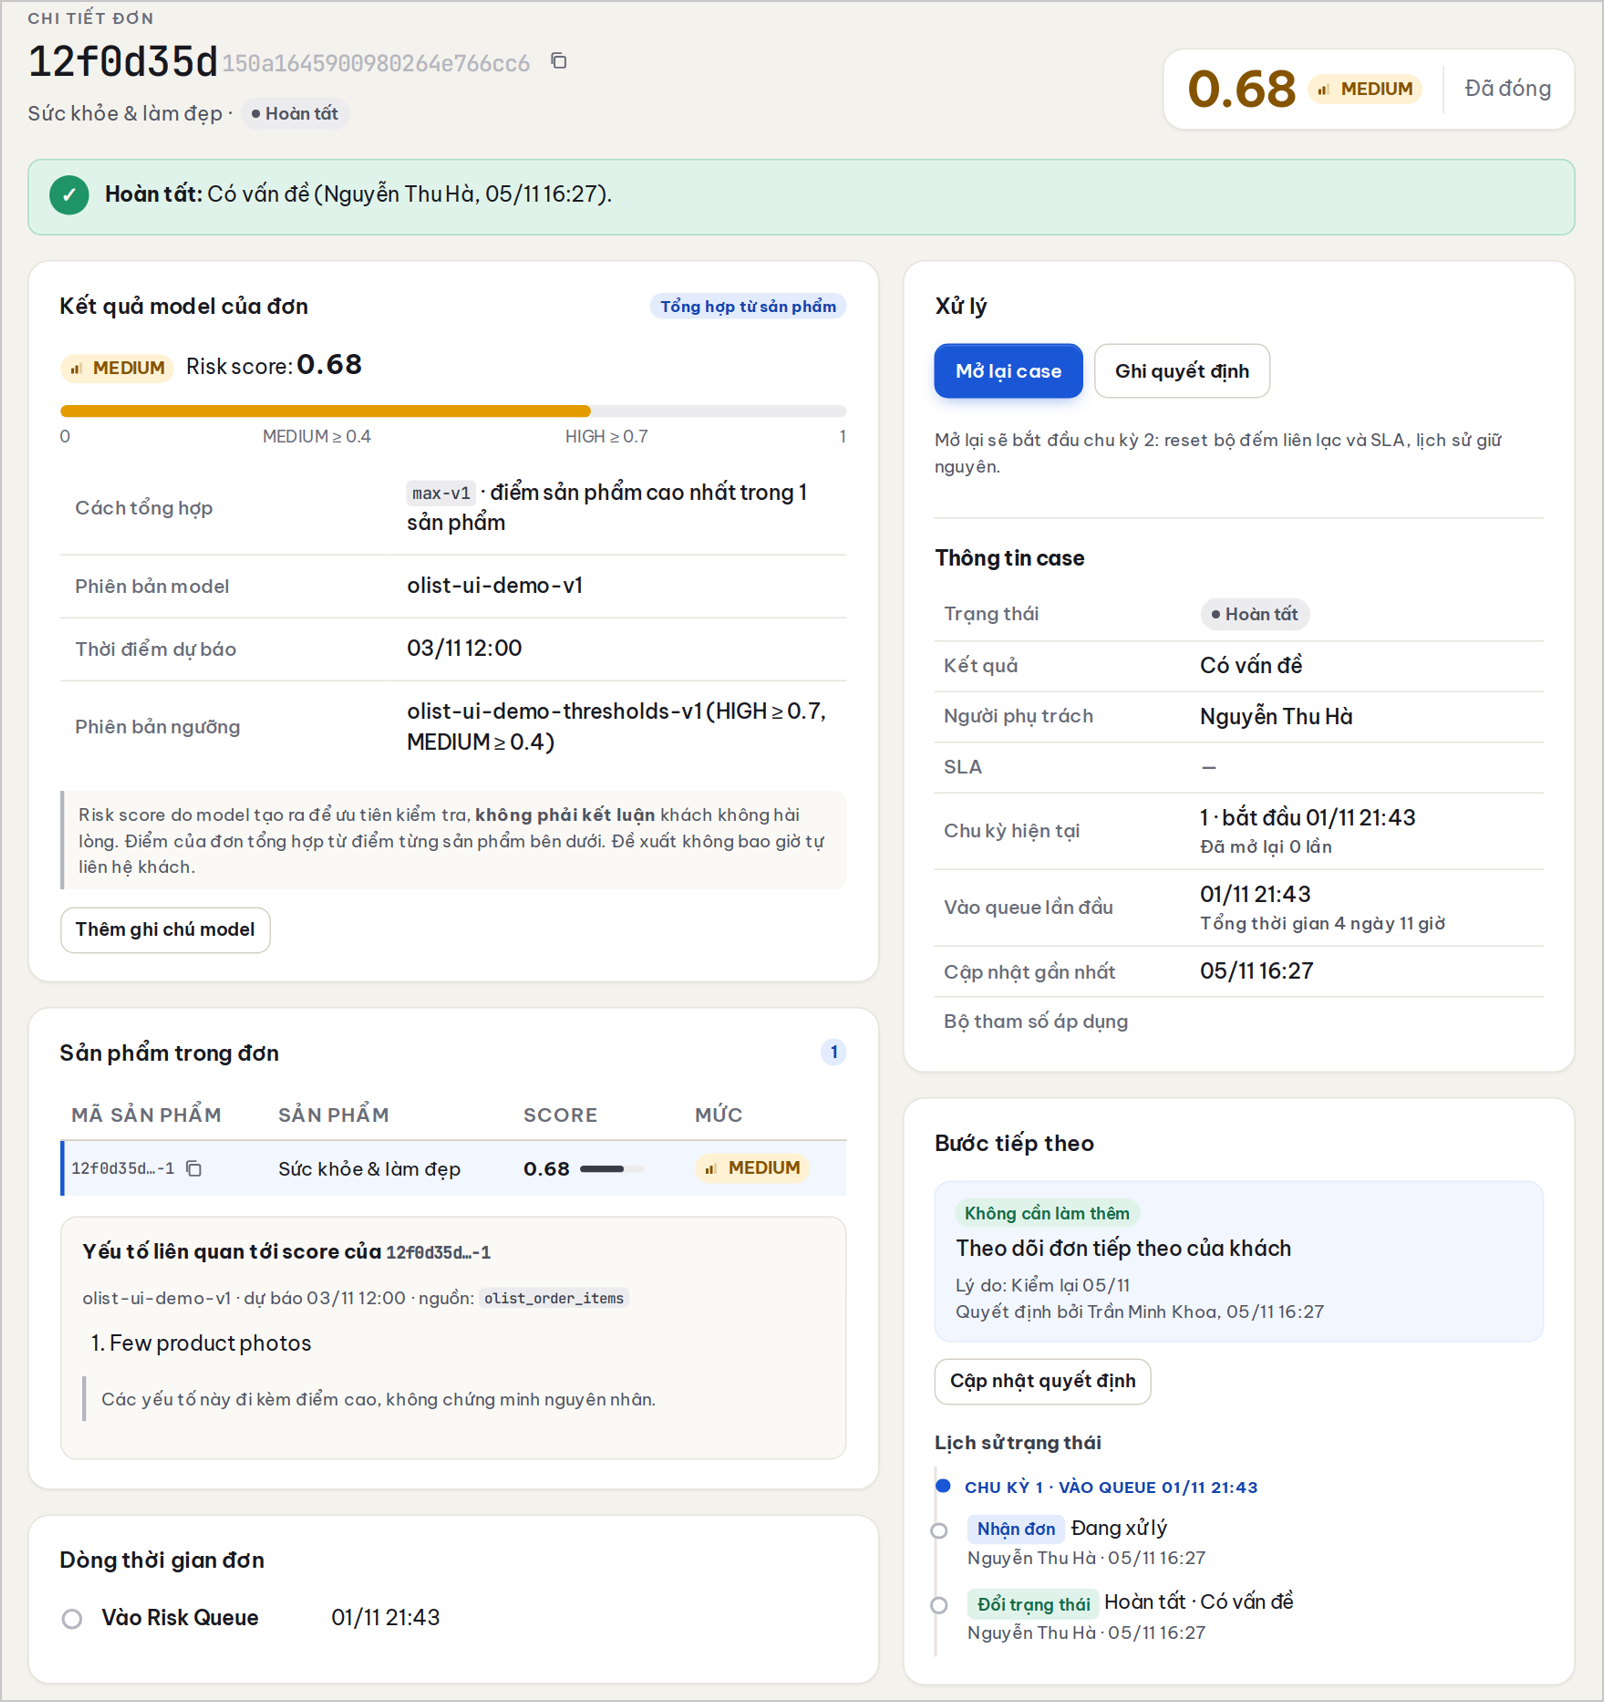
\includegraphics[width=\linewidth]{ui-closed-case}
  \caption{Case đã đóng: điểm dự báo, kết quả xử lý ``có vấn đề'' và lịch sử thao tác được lưu cùng nhau (dữ liệu demo).}\label{fig:ui-closed}
\end{figure}

\begin{figure}[htbp]\centering
\begin{tikzpicture}[font=\footnotesize, >={Latex}, node distance=0.55cm and 0.9cm,
  box/.style={draw,rounded corners,fill=#1,minimum width=3.4cm,minimum height=0.9cm,align=center}, box/.default=gray!10]
  \node[box=blue!15] (snap) {Snapshot dự đoán\\điểm, mức, phiên bản};
  \node[box=orange!20,right=of snap] (case) {Case trong\\hàng đợi ưu tiên};
  \node[box=teal!20,right=of case] (contact) {Liên hệ khách\\(các lần liên lạc)};
  \node[box=green!20,below=of contact] (outcome) {Kết quả xử lý\\có / không có vấn đề};
  \node[box=yellow!30,left=of outcome] (eval) {Cặp (điểm, kết quả)\\precision nhóm HIGH};
  \node[box=violet!20,left=of eval] (retrain) {Hiệu chỉnh, chọn ngưỡng\\hoặc huấn luyện lại};
  \node[box=red!15,below=of eval] (review) {Đánh giá sao của khách\\(nhãn $y$ ở Chương~3)};
  \draw[->] (snap) -- (case); \draw[->] (case) -- (contact); \draw[->] (contact) -- (outcome);
  \draw[->] (outcome) -- (eval); \draw[->] (review) -- (eval); \draw[->] (eval) -- (retrain);
  \draw[->,dashed] (retrain) -- node[right,font=\scriptsize]{phiên bản mới} (snap);
\end{tikzpicture}
\caption{Vòng phản hồi giữa ứng dụng và luồng học máy. Điểm số không bao giờ bị sửa; kết quả xử lý và đánh giá sao được đối chiếu với điểm gốc để đánh giá mô hình. Đường nét đứt là bước chưa được thực hiện trong đề tài.}\label{fig:feedback-loop}
\end{figure}

Ba nguyên tắc này biến ứng dụng thành điểm khởi đầu cho một thử nghiệm có đối chứng: nếu một phần đơn HIGH được chọn ngẫu nhiên để không liên hệ, dữ liệu sẵn có đủ để ước lượng tác động của việc liên hệ lên tỉ lệ đánh giá thấp, điều mà Chương~\ref{ch:method} xác định là nằm ngoài phạm vi đề tài.

% ---------------------------------------------------------------------
\subsection{Minh họa luật tổng hợp max-v1}\label{sec:demo-maxv1}

Luật max-v1 quyết định đơn nào lên đầu hàng đợi, nên cần thấy rõ nó khác cách lấy trung bình ở đâu. Bảng~\ref{tab:demo-maxv1} dùng ba đơn với điểm item \emph{giả định}, chỉ để minh họa cơ chế; mức rủi ro được gán theo ngưỡng của lần chạy rừng ngẫu nhiên đã nêu ở mục~\ref{sec:demo-limits} (mức cao từ 0,286, mức trung bình từ 0,112).

\begin{table}[htbp]\centering\small
\caption{Điểm đơn theo luật max-v1 và theo trung bình (điểm item giả định)}\label{tab:demo-maxv1}
\begin{tabular}{lp{3.4cm}cccc}
\toprule
Đơn & Điểm các item & max-v1 & Mức & Trung bình & Mức \\
\midrule
A & 0,08; 0,12; 0,41       & 0,41 & \textsc{Cao}        & 0,20 & \textsc{Trung bình} \\
B & 0,30                   & 0,30 & \textsc{Cao}        & 0,30 & \textsc{Cao} \\
C & 0,15; 0,16; 0,18; 0,20 & 0,20 & \textsc{Trung bình} & 0,17 & \textsc{Trung bình} \\
\bottomrule
\end{tabular}
\end{table}

Hình~\ref{fig:ui-multi} là một đơn ba sản phẩm trong bản demo: các item có điểm 0,93, 0,79 và 0,43, điểm của đơn là 0,93 theo max-v1, trong khi trung bình chỉ là 0,72. Giao diện đánh dấu item quyết định điểm của đơn ở dòng đầu bảng sản phẩm, nên người dùng thấy ngay điểm của đơn đến từ sản phẩm nào.

\begin{figure}[htbp]\centering
  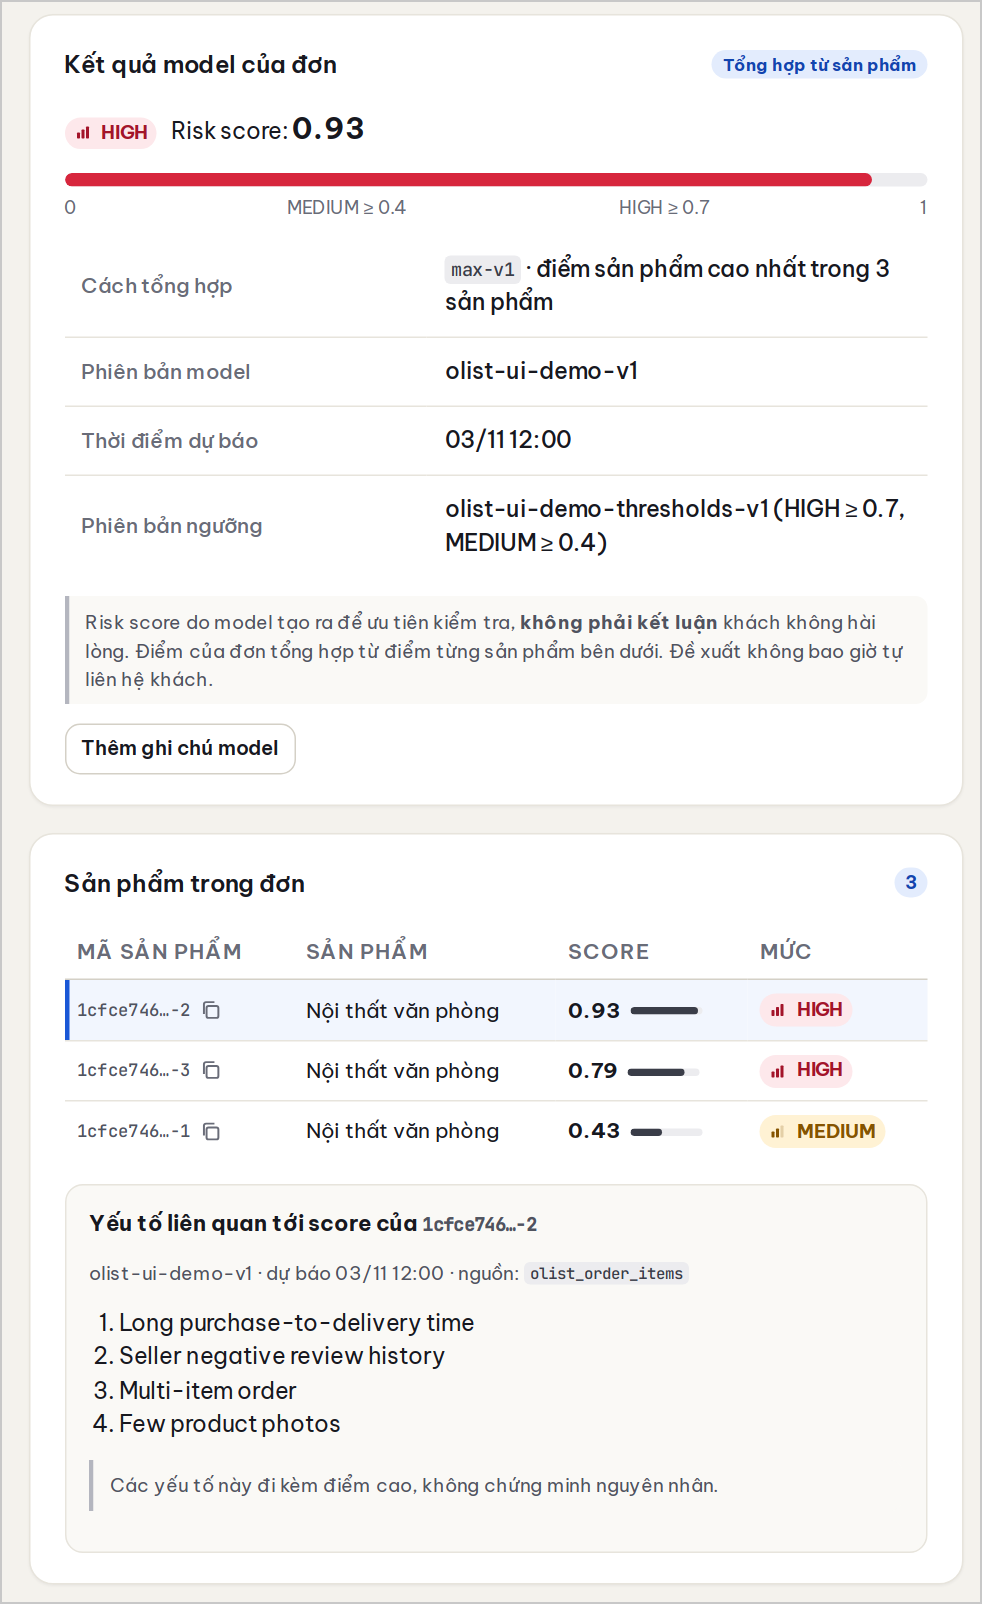
\includegraphics[width=0.62\linewidth]{ui-multi-item}
  \caption{Đơn ba sản phẩm: điểm của đơn (0,93) lấy từ item có điểm cao nhất; khối yếu tố đi kèm câu nhắc không chứng minh nguyên nhân (dữ liệu demo).}\label{fig:ui-multi}
\end{figure}

Theo max-v1, ba đơn giả định trong Bảng~\ref{tab:demo-maxv1} có thứ tự ưu tiên là A, B, C; theo trung bình, thứ tự là B, A, C. Khác biệt nằm ở đơn A: một sản phẩm có điểm 0,41 bị hai sản phẩm bình thường kéo xuống còn 0,20 nếu lấy trung bình, và đơn rơi khỏi mức cao. Đây đúng là tình huống ``mắt xích yếu nhất'' mà max-v1 được thiết kế để bắt (mục~\ref{sec:pipeline}). Đơn C cho thấy mặt trái của luật: bốn sản phẩm đều ở mức vừa phải, nhưng điểm của đơn bằng điểm cao nhất trong bốn, nên đơn nhiều sản phẩm có xu hướng được đẩy lên chỉ vì có nhiều cơ hội hơn để một item có điểm cao. Trên giao diện, cột sản phẩm cần kiểm tra (Hình~\ref{fig:ui-queue}) giúp người dùng nhận ra trường hợp này: nếu điểm của đơn đến từ một item duy nhất nổi bật, đó là tình huống A; nếu các item đều sát nhau, đó là tình huống C.

% ---------------------------------------------------------------------
\subsection{Tác động của ngưỡng lên danh sách ưu tiên}\label{sec:demo-threshold}

Bảng~\ref{tab:demo-threshold} so sánh tỉ lệ các mức rủi ro trong bản demo (ngưỡng cố định 0,7 và 0,4, đếm trên 105 case ở Hình~\ref{fig:ui-dashboard}) với tỉ lệ mà chính sách ngưỡng ở mục~\ref{sec:models} tạo ra. Vì điểm của bản demo không phải đầu ra của mô hình, bảng không so sánh hai bộ điểm mà so sánh hai \emph{cách đặt ngưỡng}.

\begin{table}[htbp]\centering\small
\caption{Tỉ lệ các mức rủi ro: ngưỡng cố định của bản demo và chính sách theo phần trăm}\label{tab:demo-threshold}
\begin{tabular}{lcccc}
\toprule
Cách đặt ngưỡng & Ngưỡng cao / trung bình & \textsc{Cao} & \textsc{Trung bình} & \textsc{Thấp} \\
\midrule
Cố định (bản demo, 105 case)        & 0,7 / 0,4         & 29\% (30) & 38\% (40) & 33\% (35) \\
Theo phần trăm (chính sách)         & $\approx$0,286 / $\approx$0,112 & 5\%  & 15\% & 80\% \\
\bottomrule
\end{tabular}
\end{table}

Ngưỡng theo phần trăm chỉ có nghĩa khi gắn với một con số năng lực cụ thể. Trong ứng dụng, con số đó là tham số vận hành do quản lý cài đặt (Hình~\ref{fig:ui-settings}): mỗi nhân viên giữ tối đa 5 đơn đang xử lý và liên hệ tối đa 3 lần mỗi chu kỳ. Với hai nhân viên trong bản demo, hệ thống xử lý cùng lúc khoảng 10 đơn, trong khi hàng đợi có 30 đơn mức cao và 40 đơn mức trung bình. Giống như mô hình và ngưỡng, mỗi thay đổi tham số tạo một phiên bản mới có thời điểm hiệu lực và lý do, nên có thể biết một đơn được xử lý dưới năng lực nào khi đánh giá về sau.

\begin{figure}[htbp]\centering
  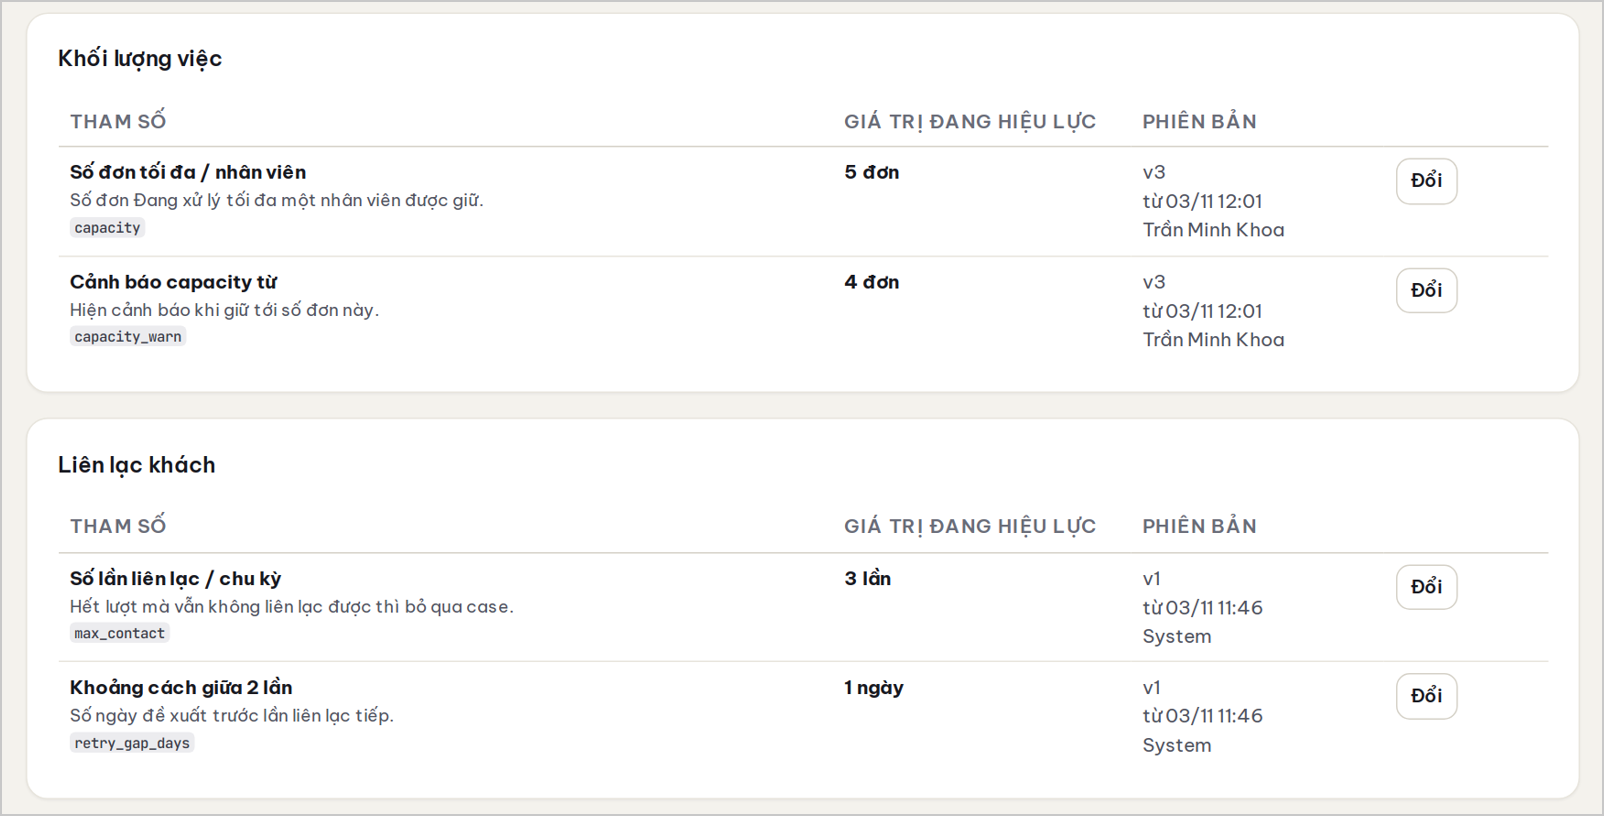
\includegraphics[width=\linewidth]{ui-settings-capacity}
  \caption{Tham số năng lực xử lý: số đơn tối đa mỗi nhân viên và số lần liên lạc mỗi chu kỳ, kèm phiên bản và thời điểm hiệu lực (dữ liệu demo).}\label{fig:ui-settings}
\end{figure}

Hai cách đặt ngưỡng cho ra hai hàng đợi rất khác nhau. Với ngưỡng cố định, gần một phần ba số đơn ở mức cao, nghĩa là quản lý phải tự phân công khoảng 30 đơn mỗi đợt thay vì khoảng 5 đơn; khi mọi thứ đều ``cao'', mức cao không còn giúp chọn ra đơn cần làm trước. Ngưỡng theo phần trăm giữ cho số đơn mức cao bằng đúng năng lực xử lý, bất kể điểm số tuyệt đối của mô hình cao hay thấp. Chiều ngược lại cũng sai: ngưỡng mức cao ghi nhận được với rừng ngẫu nhiên chỉ khoảng 0,286, nên nếu giữ ngưỡng cố định 0,7 khi thay bằng điểm thật, số đơn mức cao sẽ ít hơn nhiều so với 5\% và phần năng lực dành cho nhóm này bị bỏ trống.

% ---------------------------------------------------------------------
\subsection{Giới hạn của bản demo}\label{sec:demo-limits}

Bản demo chứng minh luồng từ điểm số đến hành động chạy được từ đầu đến cuối, nhưng chưa chứng minh mô hình mang lại giá trị trong vận hành. Có ba khoảng cách giữa bản demo và kết quả nghiên cứu:

\begin{enumerate}
  \item \textbf{Điểm số minh họa thay vì điểm của mô hình.} Mô hình rừng ngẫu nhiên được giữ lại chưa được đóng gói và đưa vào ứng dụng. Lần rà soát toàn luồng ngày 31/10/2026 ghi nhận tệp mô hình nạp được và dự đoán được khi gọi trực tiếp, nhưng không đọc được qua bộ chuyển đổi của ứng dụng vì khác định dạng đóng gói. Ngoài ra, chấm điểm chính thức trên giai đoạn kiểm tra cần chờ một tập kiểm tra chưa từng được xem, như đã nêu ở mục~\ref{sec:eval}.
  \item \textbf{Ngưỡng cố định thay vì ngưỡng theo năng lực.} Bản demo dùng ngưỡng 0,7 và 0,4. Với mô hình thật, ngưỡng được chọn theo tỉ lệ phần trăm trên phân vùng chọn ngưỡng; lần chạy rừng ngẫu nhiên trước đó ghi nhận ngưỡng mức cao khoảng 0,286 và mức trung bình khoảng 0,112 (mục~\ref{sec:demo-threshold}).
  \item \textbf{Chưa có giải thích mô hình.} Khối yếu tố rủi ro trên giao diện đã có chỗ, nhưng chưa có lần tính SHAP nào được lưu, nên nhân viên chỉ thấy điểm mà chưa thấy lý do.
\end{enumerate}

Nhờ ứng dụng chỉ đọc bảng dự đoán, cả ba khoảng cách này đều được xử lý ở phía luồng học máy: chấm điểm bằng mô hình thật, ghi ngưỡng tương ứng vào bảng ngưỡng và bổ sung yếu tố rủi ro vào snapshot mới. Giao diện và quy trình xử lý không cần thay đổi.
